
El desarrollo de la Teor'ia de Conjuntos de Cantor y, en general, de las matem'aticas en el siglo \textsc{xix} dio lugar a muchos argumentos que hoy conocemos como \enquote{diagonales}. Veamos, como ejemplo, el siguiente teorema.

\begin{teo*}[Teorema de la Diagonal de Cantor]
El intervalo real unitario $(0,1)$ no es numerable. Es decir, no existe una biyección $\ff{\phi}{\N}{(0,1)}$.
\end{teo*}

\begin{proof}
Procederemos por reducción al absurdo. Supongamos que el conjunto es numerable y que, por tanto, existe una biyección $\phi$ que nos permite enlistar exhaustivamente todos los elementos del intervalo como una sucesión $x_1, x_2, x_3, \dots$, donde $x_n = \phi(n)$.

Podemos representar cada número $x_n$ mediante su expansión decimal única:
\begin{align*}
    x_1 &= 0.a_{11} a_{12} a_{13} a_{14} \dots \\
    x_2 &= 0.a_{21} a_{22} a_{23} a_{24} \dots \\
    x_3 &= 0.a_{31} a_{32} a_{33} a_{34} \dots \\
    &\vdotswithin{=} \\
    x_n &= 0.a_{n1} a_{n2} a_{n3} a_{nn} \dots 
\end{align*}
Nuestro objetivo es encontrar un número real $y \in (0,1)$ que no se encuentre en dicha lista. Definimos $y = 0.d_1d_2d_3\dots$ determinando cada dígito decimal $d_n$ en función de la diagonal de nuestra lista (los términos $a_{nn}$). La regla de construcción es la siguiente:
\[
    d_n = \begin{cases} 
    1 & \text{si } a_{nn} \neq 1 \\
    2 & \text{si } a_{nn} = 1 
    \end{cases}
\]
Analicemos el resultado. Para cualquier índice $n \in \N$, el $n$-ésimo dígito de nuestro nuevo número $y$ difiere del $n$-ésimo dígito del número $x_n$ de la lista (es decir, $d_n \neq a_{nn}$). 

Esto implica necesariamente que $y \neq x_n$ para todo $n$. Sin embargo, $y$ es un número real bien definido con expansión decimal de unos y dos, por lo que $y \in (0,1)$. Hemos encontrado un elemento que escapa a la enumeración $\phi$, contradiciendo la hipótesis de que $\phi$ era sobreyectiva.
\end{proof}

Podemos observar en la demostración anterior que, para construir el elemento $y$, recurrimos explícitamente a la diagonal principal de la matriz; es decir, nos fijamos en los términos de la forma $a_{nn}$.

\begin{center}
\tikzset{every picture/.style={line width=0.75pt}}

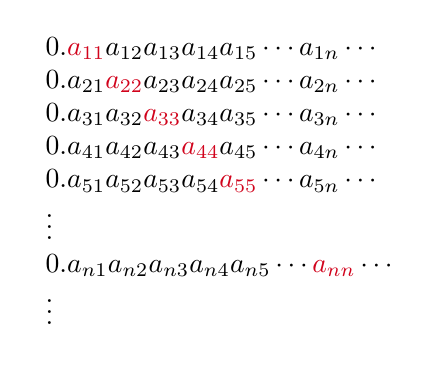
\begin{tikzpicture}[x=0.75pt,y=0.75pt,yscale=-1,xscale=1]
% Text Node
\draw (215,31.4) node [anchor=north west][inner sep=0.75pt]    {$ \begin{array}{l}
0.\textcolor[rgb]{0.82,0.01,0.11}{a_{11}} a_{12} a_{13} a_{14} a_{15} \cdots a_{1n} \cdots \\
0.a_{21}\textcolor[rgb]{0.82,0.01,0.11}{a_{22}} a_{23} a_{24} a_{25} \cdots a_{2n} \cdots \\
0.a_{31} a_{32}\textcolor[rgb]{0.82,0.01,0.11}{a_{33}} a_{34} a_{35} \cdots a_{3n} \cdots \\
0.a_{41} a_{42} a_{43}\textcolor[rgb]{0.82,0.01,0.11}{a_{44}} a_{45} \cdots a_{4n} \cdots \\
0.a_{51} a_{52} a_{53} a_{54}\textcolor[rgb]{0.82,0.01,0.11}{a_{55}} \cdots a_{5n} \cdots \\
\vdots \\
0.a_{n1} a_{n2} a_{n3} a_{n4} a_{n5} \cdots \textcolor[rgb]{0.82,0.01,0.11}{a_{nn}} \cdots \\
\vdots 
\end{array}$};
\end{tikzpicture}
\end{center}

La clave del argumento reside en el uso de esta información diagonal para definir un objeto que difiere sistemáticamente de todos los elementos listados. Nótese que el éxito de la construcción depende de la capacidad de \enquote{invertir} el valor encontrado en la diagonal. El apelar a esta estructura es lo que conocemos hoy como \textbf{argumento diagonal}.

Sin embargo, este esquema lógico es generalizable y trasciende la geometría de una matriz infinita. En muchos contextos, la diagonal no es tan visible, pero el mecanismo subyacente es el mismo: la \textbf{autorreferencia}. 

Si trasladamos este procedimiento a la Teoría de Conjuntos, sustituyendo la indexación numérica por la relación de pertenencia, el argumento diagonal deja de producir \enquote{nuevos elementos} para revelar, en su lugar, contradicciones en la estructura misma de la teoría. Fue precisamente al aplicar este principio de diagonalización sobre la totalidad de los conjuntos que Bertrand Russell formuló, en 1901, la siguiente paradoja.

\begin{teo*}
No existe una biyecci'on entre el conjunto de los n'umeros naturales, $\mathbb {N}$, y el intervalo real $(0,1)$.    
\end{teo*}
\begin{proof}
    Supongamos por el contrario que s'i existe una biyecci'on. Entonces hay una funci'on $\phi: 
    \N \to (0,1)$ que enumera a todos los n'umeros reales en el intervalo $(0,1)$. Es decir, podemos enlistar a todos los n'umeros del intervalo, 

    
    \begin{align*}
        &0.a_{00}a_{01}a_{02}a_{03}\dots\\
        &0.a_{10}a_{11}a_{12}a_{13}\dots\\
        &0.a_{20}a_{21}a_{22}a_{23}\dots\\
        &\vdots\\
        &0.a_{n0}a_{n0}a_{n2}a_{n3}\dots \\
        &\vdots
    \end{align*}
    donde $a_{ij}\in \{0,1,2,3,4,5,6,7,8,9\}$ para todo $i,j\in \N$. De esta forma tenemos una matriz infinita donde los renglones de ésta constituyen los elementos en el intervalo. Buscamos ahora construir un elemento en $(0,1)$ que no est'e en esta lista. Para ello, consideremos las entradas $a_{ij}$ tales que $i=j$. Si $a_{ii} = 2$, definimos $b_i = 1$. Si $a_{ii}\neq 2$, definimos $b_i=2$. Afirmamos que el n'umero $b=0.b_1b_2b_3b_4\dots$ no est'a en la lista, i.e., no es un elemento de la imagen  de $\phi$. Para ver eso, basta observar que si $b$ estuviese en la lista, existir'ia un $n
    \in \N$ tal que $\phi(n) = b$. Pero $b_n$ ser'ia un dígito distinto a $a_{nn}$ pues construimos a $b$ de tal forma que fuese distinto en dicha entrada. Como los dos n'umeros son diferentes en ese decimal, no pueden ser el mismo n'umero y por tanto $\phi(n)\neq b$. Hemos entonces construido un elemento que no est'a en la imagen de $\phi$ pero que s'i est'a en $(0,1)$. Pero supusimos que $\phi$ es biyectiva por lo que en particular es suprayectiva. Esta es una clara contradicci'on, por lo que concluimos que no puede existir una funci'on biyectiva entre $\N$ y $(0,1)$.      
\end{proof}

Podemos observar en la demostración anterior que, para construir el elemento $y$, recurrimos explícitamente a la diagonal principal de la matriz; es decir, nos fijamos en los términos de la forma $a_{nn}$.

\begin{center}
\tikzset{every picture/.style={line width=0.75pt}}

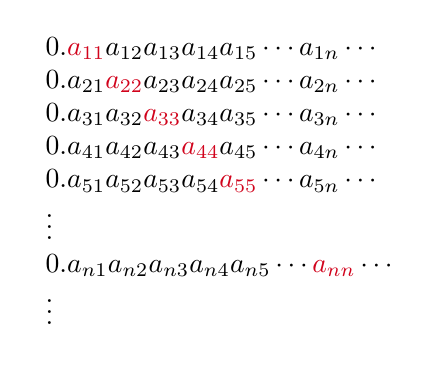
\begin{tikzpicture}[x=0.75pt,y=0.75pt,yscale=-1,xscale=1]
% Text Node
\draw (215,31.4) node [anchor=north west][inner sep=0.75pt]    {$ \begin{array}{l}
0.\textcolor[rgb]{0.82,0.01,0.11}{a_{11}} a_{12} a_{13} a_{14} a_{15} \cdots a_{1n} \cdots \\
0.a_{21}\textcolor[rgb]{0.82,0.01,0.11}{a_{22}} a_{23} a_{24} a_{25} \cdots a_{2n} \cdots \\
0.a_{31} a_{32}\textcolor[rgb]{0.82,0.01,0.11}{a_{33}} a_{34} a_{35} \cdots a_{3n} \cdots \\
0.a_{41} a_{42} a_{43}\textcolor[rgb]{0.82,0.01,0.11}{a_{44}} a_{45} \cdots a_{4n} \cdots \\
0.a_{51} a_{52} a_{53} a_{54}\textcolor[rgb]{0.82,0.01,0.11}{a_{55}} \cdots a_{5n} \cdots \\
\vdots \\
0.a_{n1} a_{n2} a_{n3} a_{n4} a_{n5} \cdots \textcolor[rgb]{0.82,0.01,0.11}{a_{nn}} \cdots \\
\vdots 
\end{array}$};
\end{tikzpicture}
\end{center}

La clave del argumento reside en el uso de esta información diagonal para definir un objeto que difiere sistemáticamente de todos los elementos listados. Nótese que el éxito de la construcción depende de la capacidad de \enquote{invertir} el valor encontrado en la diagonal. El apelar a esta estructura es lo que conocemos hoy como \textbf{argumento diagonal}.

Sin embargo, este esquema lógico es generalizable y trasciende la geometría de una matriz infinita. En muchos contextos, la diagonal no es tan visible, pero el mecanismo subyacente es el mismo: la \textbf{autorreferencia}. 

Si trasladamos este procedimiento a la Teoría de Conjuntos, sustituyendo la indexación numérica por la relación de pertenencia, el argumento diagonal deja de producir \enquote{nuevos elementos} para revelar, en su lugar, contradicciones en la estructura misma de la teoría. Fue precisamente al aplicar este principio de diagonalización sobre la totalidad de los conjuntos que Bertrand Russell formuló, en 1901, la siguiente paradoja.

Podemos observar en la demostraci'on del teorema anterior que para construir al elemento $b$ usamos la diagonal principal de la matriz, i.e., nos fijamos en los elementos de la forma $a_{ii}$. 


\begin{center}
\tikzset{every picture/.style={line width=0.75pt}} %set default line width to 0.75pt        

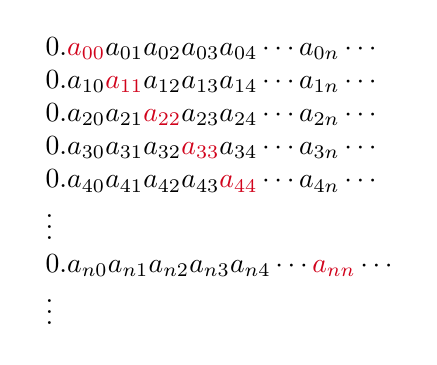
\begin{tikzpicture}[x=0.75pt,y=0.75pt,yscale=-1,xscale=1]
%uncomment if require: \path (0,300); %set diagram left start at 0, and has height of 300


% Text Node
\draw (215,31.4) node [anchor=north west][inner sep=0.75pt]    {$ \begin{array}{l}
0.\textcolor[rgb]{0.82,0.01,0.11}{a_{00}} a_{01} a_{02} a_{03} a_{04} \cdots a_{0n} \cdots \\
0.a_{10}\textcolor[rgb]{0.82,0.01,0.11}{a_{11}} a_{12} a_{13} a_{14} \cdots a_{1n} \cdots \\
0.a_{20} a_{21}\textcolor[rgb]{0.82,0.01,0.11}{a_{22}} a_{23} a_{24} \cdots a_{2n} \cdots \\
0.a_{30} a_{31} a_{32}\textcolor[rgb]{0.82,0.01,0.11}{a_{33}} a_{34} \cdots a_{3n} \cdots \\
0.a_{40} a_{41} a_{42} a_{43}\textcolor[rgb]{0.82,0.01,0.11}{a_{44}} \cdots a_{4n} \cdots \\
\vdots \\
0.a_{n0} a_{n1} a_{n2} a_{n3} a_{n4} \cdots \textcolor[rgb]{0.82,0.01,0.11}{a_{nn}} \cdots \\
\vdots 
\end{array}$};


\end{tikzpicture}
\end{center}

El apelar a esta diagonal principal de la matriz para llegar a nuestra prueba es lo que conocemos como un \emph{argumento diagonal}. De hecho, este resultado es conocido como el \textit{argumento de la diagonal de Cantor}.

Los argumentos diagonales usualmente no son provistos de una manera tan expl'icita como en el argumento de Cantor. En realidad, muchos de estos son m'as conocidos por presentar en su desarrollo, visto metamatem'aticamente, la noci'on de autoreferencia. Para ver esto, consideremos la siguiente,

%\textbf{Paradoja de Russel:}
\subsubsection*{Paradoja de Russell}

La paradoja de Russell concierne a la teor'ia de conjuntos informal, en donde cualquier propiedad define un conjunto. Para ver la paradoja, es necesario considerar a los conjuntos que se pertenecen a s'i mismos, i.e., pensemos en todos los conjuntos $X$ tales que $X\in X$. Consideremos ahora el siguiente conjunto: 
\[R = \{X\vert X\notin X\}\]
Es decir, $R$ es el conjunto de todos los conjuntos que no se pertenecen a s'i mismos. Surge entonces la pregunta, ¿$R$ se pertenece a s'i mismo? Si $R\in R$ entonces tenemos $R\notin R$ por definici'on de $R$. Por otro lado, si $R\notin R$ entonces es un conjunto que no se pertenece a s'i mismo y por tanto $R\in R$. Podemos observar entonces que en ambos casos llegamos a 
\[R\in R \iff R\notin R\]
Esta es una clara contradicci'on, por lo que llegamos a una paradoja. 

La Paradoja de Russell nos deja ver la necesidad de formalizar la teor'ia de conjuntos y que no puede ser el caso de que cualquier propiedad defina a un conjunto. De hacerlo, nuestra teor'ia se derrumbar'ia. 

En el coraz'on de la paradoja de Russell est'a la autoferencia. Construimos un conjunto $R$ tal que al considerarse a s'i mismo lleva a una paradoja. Esta paradoja es otro ejemplo de un argumento diagonal. Dicho esto, podemos ver que en ning'un momento construimos una matriz ni apelamos a una diagonal. ¿Cómo es entonces que éste es un argumento diagonal? 

Pensemos en todos los conjuntos existentes. Organiz'emoslos tanto de manera vertical como horizontal, i.e., 

\begin{align*}
    &\quad A\quad B \quad C \quad D \quad \cdots\\
    &A\\
    &B\\
    &C\\
    &D\\
    &\vdots
\end{align*}
Asignemos valores como sigue: si el elemento horizontal pertenece al elemento vertical, ponemos un $1$. En caso contrario, ponemos un $0$. As'i por ejemplo supongamos que $A\in B$ y que $A\notin A$, tendr'iamos entonces 

\begin{align*}
    &\,\,\quad A\quad B \quad C \quad D \quad \cdots\\
    &A\quad 0\\
    &B\quad 1\\
    &C\\
    &D\\
    &\vdots
\end{align*}

Nuestra matriz entonces podr'ia lucir algo como el siguiente ejemplo, 
\[
\begin{matrix}
    & A & B & C & D & E & F & \dots\\
    A &  0 & 0 & 0 &1 & 0 &1 & \dots\\
    B & 1 & 1 & 0 &1 &  0 & 0 & \dots\\
    C&  1 & 0 & 0 & 1 & 1 & 1 & \dots\\
    D& 0 & 0 & 1 & 0 & 1 & 1 & \dots \\
    E& 1 & 0 & 1 & 0 &1 & 0 & \dots\\
    F& 1 & 1 & 0 & 0 & 1 & 0 & \dots\\
    \vdots & \vdots & \vdots & \vdots & \vdots & \vdots & \vdots & \ddots\\
\end{matrix}\]
Aquí, nos interesan los valores de la diagonal principal. Las entradas $0$ son los $X$ tales que $X\notin X$ y la teor'ia informal de conjuntos nos dice que podemos crear el conjunto de todos los conjuntos cuyo valor en esta diagonal principal es $0$. Siendo este un conjunto, ocupa un lugar en esta matriz. ¿Qué valor tiene $R$ en esta diagonal principal? Como vimos, vale $0$ si y sólo si vale $1$. La existencia de este conjunto, entonces, nos lleva a un absurdo, por lo que concluimos que tal conjunto no puede existir. Como la teoría informal de conjuntos permite la construcción de dicho conjunto, podemos ver que existe un problema fundamental con ésta.

Esta construcci'on nos permite ver que en un problema de autoreferencia permite ser representado en forma de un elemento de la diagonal principal. En s'i, entendemos que la $n-$'esima columna est'a \emph{hablando algo} de la $n-$'esima fila, es decir, en cierto modo pensamos que est'a \emph{hablando algo de s'i mismo} al compartir este valor $n$ en com'un. 

De estos casos de autoreferencia uno de los m'as famosos y el m'as rodeado de inter'es filos'ofico es el primer teorema de incompletitud de Gödel. Un planteamiento y demostraci'on formal de 'este teorema ocupar'ia demasiado espacio y saldr'ia mucho del inter'es de 'esta introducci'on, por lo que nos limitaremos dar una explicaci'on breve del teorema, en un esbozo que sigue al dado por Gödel en \parencite{gdl}.

\section*{La Paradoja de Russell}

La Paradoja de Russell concierne a la llamada \textit{Teoría Intuitiva de Conjuntos} (o \textit{Naive Set Theory}), la cual se fundamentaba en el principio de que cualquier propiedad lógica define un conjunto. Para visualizar el conflicto, es necesario considerar conjuntos que puedan pertenecerse a sí mismos (por ejemplo, el conjunto de \enquote{todas las ideas} es, en sí mismo, una idea).

Consideremos el conjunto $R$, definido como la colección de todos los conjuntos que \textbf{no} son elementos de sí mismos:
\[R = \{X \mid X \notin X\}\]
Surge entonces la pregunta inevitable: ¿Se pertenece $R$ a sí mismo?
Analicemos las dos posibilidades:
\begin{itemize}
    \item Si $R \in R$, entonces debe cumplir la condición que define al conjunto, es decir, $R \notin R$.
    \item Si $R \notin R$, entonces cumple la condición de entrada, por lo que debería estar dentro, es decir, $R \in R$.
\end{itemize}
En ambos casos llegamos a la contradicción:
\[R \in R \iff R \notin R\]
Este resultado evidencia que la teoría intuitiva es inconsistente: no puede ser el caso que cualquier propiedad defina un conjunto. De permitirlo, el edificio lógico de la teoría se derrumbaría.

Ahora bien, hemos afirmado que en el corazón de esta paradoja reside la \textbf{autorreferencia} y que se trata de un argumento diagonal. Sin embargo, en la formulación anterior no construimos ninguna matriz ni apelamos a dígitos decimales. ¿Cómo justificamos entonces que este es el mismo fenómeno que observamos con Cantor?

Imaginemos, bajo la hipótesis de la teoría intuitiva, que podemos listar \enquote{todos los conjuntos existentes}. Organicémoslos tanto vertical como horizontalmente para formar una tabla de pertenencia:

\begin{center}
$ \begin{matrix} 
& A & B & C & D & \dots \\
A & \cdot & \cdot & \cdot & \cdot & \\
B & \cdot & \cdot & \cdot & \cdot & \\
C & \cdot & \cdot & \cdot & \cdot & \\
\vdots & & & & & \ddots
\end{matrix} $
\end{center}

Asignemos valores de verdad a las intersecciones: pondremos un $1$ si el conjunto de la fila pertenece al conjunto de la columna, y un $0$ en caso contrario. Supongamos, por ejemplo, que $A \notin A$ (diagonal es 0), $A \in B$, etc. Nuestra matriz de incidencia luciría así:


\begin{center}
\tikzset{every picture/.style={line width=0.75pt}}

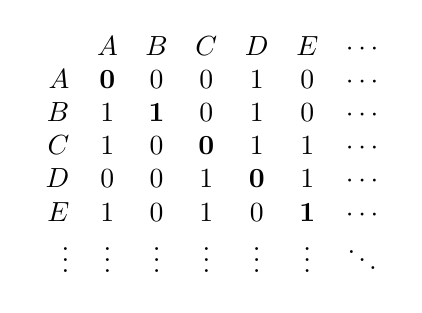
\begin{tikzpicture}[x=0.75pt,y=0.75pt,yscale=-1,xscale=1]
% Text Node
\draw (215,31.4) node [anchor=north west][inner sep=0.75pt]    {$
\begin{array}{rcccccc}
    & A & B & C & D & E & \cdots \\
  A & \mathbf{0} & 0 & 0 & 1 & 0 & \cdots \\
  B & 1 & \mathbf{1} & 0 & 1 & 0 & \cdots \\
  C & 1 & 0 & \mathbf{0} & 1 & 1 & \cdots \\
  D & 0 & 0 & 1 & \mathbf{0} & 1 & \cdots \\
  E & 1 & 0 & 1 & 0 & \mathbf{1} & \cdots \\
  \vdots & \vdots & \vdots & \vdots & \vdots & \vdots & \ddots
\end{array}
$};
\end{tikzpicture}
\end{center}



Al igual que en el teorema anterior, nuestra atención se centra en la \textbf{diagonal principal} (marcada en negritas). Las entradas con valor $0$ en la diagonal corresponden a los conjuntos $X$ tales que $X \notin X$.
La definición de $R$ es precisamente la instrucción de tomar esos casos: $R$ se define \enquote{invirtiendo} la diagonal principal.
\[ X \in R \iff \text{Diagonal}(X, X) = 0 \]
Dado que $R$ es un conjunto dentro de esta teoría, debe ocupar algún lugar en la lista (digamos, una fila $R$). ¿Qué valor tiene $R$ en su propia intersección diagonal? Por construcción, debe tener el valor opuesto al que tiene en la diagonal. Es decir, el valor en $(R, R)$ debe ser $0$ si y solo si es $1$.

Esta visualización confirma que la paradoja es estructuralmente idéntica al argumento de Cantor: el problema surge al intentar introducir dentro de la matriz un objeto definido por la negación de la diagonal de dicha matriz.

\subsection*{El Teorema de Incompletitud de Gödel}

De estos casos de autorreferencia, el más célebre y con mayor peso filosófico es el \textbf{Primer Teorema de Incompletitud de Gödel}. Un planteamiento y demostración rigurosa de este teorema ocuparía demasiado espacio y se saldría de los objetivos de esta introducción. Por ello, nos limitaremos a dar un esbozo que sigue la línea argumental presentada por el propio Gödel en \cite{gdl}, resaltando cómo es, en el fondo, otro argumento diagonal.

La idea central y genial de Gödel fue trasladar el problema de la autorreferencia al lenguaje de la aritmética. Para ello, ideó un método de codificación (conocido como \textit{numeración de Gödel}) que asigna a cada fórmula $\phi$ un número natural único, denotado por $\ulcorner \phi \urcorner$. Esto permite que la aritmética \enquote{hable} de sus propias fórmulas.

Gracias a esta codificación, la propiedad metamatemática \enquote{$y$ es una demostración de $x$} se puede expresar como una relación aritmética, llamémosla $\dems(x,y)$. A partir de aquí, podemos definir el concepto de ser demostrable como 

$$\dems(x) \iff \exists y \dems(x,y).$$

A partir de aquí aparece la diagonal como en los otros dos ejemplos. Gödel definió una función de sustitución, $s(n, m)$, que calcula el código de la fórmula resultante al tomar la fórmula con código $n$ y reemplazar su variable libre por el número $m$, es decir, 
\[ s(\ulcorner \phi(x) \urcorner, m) = \ulcorner \phi(m) \urcorner. \]
Esta función $s$ es la herramienta que nos permite \enquote{caminar por la diagonal}: si evaluamos $s(n, n)$, estamos pidiéndole intrínsecamente a la fórmula número $n$ que hable del número $n$. Es el análogo aritmético de mirar la entrada $(n,n)$ en la matriz del argumento de la diagonal de Cantor o en la matriz que visualizamos de pertencencia para la Paradoja de Russell.

Ahora, consideremos la siguiente fórmula:
\[ P(x) := \neg \dems( s(x, x) ). \]
Sea $k$ el número de Gödel de esta fórmula, es decir, $k = \ulcorner P(x) \urcorner$. Si evaluamos ahora la diagonal en este punto (calculamos $P(k)$), obtenemos una sentencia $G$ tal que:
\[ G \iff \neg \dems( s(k, k) ) \]
Pero por definición de nuestra función de sustitución, $s(k, k)$ es precisamente el código de $G$. Es decir, $\ulcorner G \urcorner = s(k, k)$. Sustituyendo esto, llegamos a:
\[ G \iff \neg \dems( \ulcorner G \urcorner ) \]
Esta sentencia $G$ afirma, literalmente: \enquote{yo no soy demostrable}.

Si el sistema es consistente, no puede demostrar falsedades, por lo que no puede demostrar $G$ (ya que si lo hiciera, $G$ sería falsa). Pero al no poder demostrarla, lo que $G$ afirma es verdad. Tenemos entonces una sentencia que es verdadera pero no demostrable dentro del sistema.

Este resultado, al igual que los de Cantor y Russell, surge de la capacidad de construir un objeto que niega su propia posición en la diagonal del sistema. El propósito de este trabajo es mostrar cómo la Teoría de Categorías, y en particular el Teorema de Lawvere, unifica todos estos argumentos bajo un mismo principio estructural.

\textbf{Primer Teorema de Incompletitud de Gödel}

Los sistemas formales que proveen los Axiomas de Peano o los de Zermelo-Fraenkel, que son capaces de construir aritmética básica de los naturales, tienen limitaciones internas respecto a qué pueden demostrar. Es decir, existen proposiciones en dichos sistemas que no pueden ser demostradas ni refutadas. Añadir estas proposiciones como axiomas no resolvería el problema: en este nuevo sistema existir'ian tambi'en proposiciones indecidibles, i.e., ni demostrables ni refutables. Este problema no es exclusivo a los dos sistemas mencionados, como veremos en el cap'itulo 3, una cantidad extensiva de sistemas formales de este tipo son incompletos, en el sentido de que tendr'an proposicones indecidibles. Es importante observar que estas proposiciones indecidibles ocurren tambi'en porque suponemos que estos sistemas son consistentes, una hipótesis necesaria para más adelante.

El argumento heurístico que provee Gödel, y que nos permitirá exhibir la diagonalidad del argumento, nace con la idea de que en un sistema formal, es inconsecuente qué signos son ocupados para describir el sistema. Es decir, la elección de símbolos como paréntesis \enquote{$()$}, conectivos l'ogicos \enquote{$\lor$}, \enquote{$\land$}, etc. es arbitraria y, por tanto, es igual de plausible usar números naturales en su lugar. De esta forma, fórmulas en nuestro sistema se convierten en sucesiones finitas de números naturales y demostraciones se vuelven sucesiones finitas de sucesiones finitas de números naturales. 

Lo increíble de esta idea es que vuelve problemas metamatemáticos, es decir, problemas que nosotros observamos respecto al sistema, en problemas de números naturales. Por ejemplo, si nosotros usamos el número $0$ en lugar del conectivo lógico $\lor$, entonces una fórmula como \enquote{$x = 0$} en el sistema se puede entender tambi'en a nivel metamatem'atico como \enquote{$x= \lor$}. Es entonces posible construir dentro del sistema una fórmula $F(v)$, donde $v$ es una sucesión finita de números, que a nivel metamatemáticos nos diga \enquote{$v$ es una f'ormula demostrable}. En su demostraci'on, Gödel construye $40$ funciones recursivas para llegar a ésta fórmula. Esta fórmula es el interés principal de hacer estos cambios de simbología. 

Ahora, para el objetivo en mano, nos concentraremos en fórmulas bien formadas con una sola variable libre, por ejemplo, como la provista arriba \enquote{$x=0$}. Podemos imaginar estas f'ormulas con una sola variable libre ordenadas en una sucesi'on, de modo que sean fácilmente identificables. En esta sucesión, denotamos a la $n-$'esima entrada por $R_n$. 

Representamos por $\sub(R_n, m)$ a la f'ormula derivada de sustitur todas las instancias de la 'unica variable libre en $R_n$ por el n'umero natural $m$. A su vez, si una fórmula es demostrable, lo denotamos por $\dems (F)$. Observemos que esto 'ultimo es la f'ormula mencionada arriba por la cual surge esta necesidad de una numeraci'on de los s'imbolos, f'ormulas, etc.  Con estas notaciones en mano, definimos el siguiente conjunto $K$: 

\[K = \{n\in \N \vert \lnot \dems(\sub(R_n,n))\}\]

Es decir, los elementos en $K$ son los naturales $n$ tales que la f'ormula resultante de substituir todas las entradas de la variable libre en la f'ormula $R_n$ (que es una f'ormula con una sola variable libre) no es demostrable en el sistema formal. 

Las nociones que conforman a este conjunto ($R_n$, $\dems$, $\sub$) son todas definibles en el sistema, por lo que la noci'on de pertenencia al conjunto $K$ es tambi'en definible dentro del sistema. Es decir, existe una f'ormula  de una sola variable libre, $S$, tal que 
\[\dems(\sub(S,n))\iff n\in K\]

Al ser una f'ormula de una sola variable libre, tiene un lugar en la secuencia, por lo que hay un $g\in \N$ para el cual $S=R_g$. Llegados a este punto tenemos ya en nuestras manos una proposici'on que no es ni demostrable ni refutable en el sistema, a saber 
\[\sub(R_g,g)\]

Antes de ver por qu'e no es demostrable ni refutable esta proposici'on, observemos del esbozo dado la presencia de un argumento diagonal. Por un lado, podemos acomodar en columnas a todas las f'ormulas de una sola variable libre y por otro, en filas a todos los n'umeros $n$. De ah'i podemos asignar $f$ a la entrada con f'ormula $R_n$ y n'umero $m$ si la f'ormula $\sub(R_n, m)$ no es demostrable en el sistema y $v$ si, por el contrario, es demostrable. Nuestra matriz entonces podr'ia lucir algo como 

\[
\begin{matrix}
    & R_1 & R_2 & R_3 & \dots & R_{n-1} & R_n & \dots\\
    1 &  f & f & f &f & v &v & \dots\\
    2 & f & v & v &v &  f & v & \dots\\
    3 &  v & v & f & v & f & f & \dots\\
    \vdots& \vdots & \vdots & \vdots & \vdots & \vdots & \vdots & \ddots \\
    n-1& v & v & v & v &v & v & \dots\\
    n& f & v & f & v & v & f & \dots\\
    \vdots & \vdots & \vdots & \vdots & \vdots & \vdots & \vdots & \ddots\\
\end{matrix}\]

Nuestro conjunto $K$ ser'ian los $n\in \N$ para los cuales el valor de la $n-$'esima fila en la diagonal principal son $f$. Entonces, ¿cuál será el valor que presente el número $g$ en la diagonal principal? Sale a la luz la similitud con la paradoja de Russell a través de esta visualización de la matriz. Por supuesto, aqu'i no lidiamos con una paradoja, sino con una limitaci'on de nuestro sistema. 

Retomando el esbozo de la demostraci'on, veamos por que $\sub(R_g,g)$ no es demostrable ni refutable. 

Primero, de ser demostrable, tendr'iamos que $\dems(\sub(R_g,g))$ y, por tanto, $g\notin K$. Pero $S= R_g$ y $S$ es tal que $\dems(\sub(S, g))\iff g\in K$, por lo que tendr'iamos $g\in K \iff g\notin K$. Esto es una clara contradicci'on, pues suponemos que nuestro sistema es consistente, por lo que no puede ser demostrable.

Segundo, de ser refutable, tendr'iamos que $\lnot \dems(\sub(R_g,g))$ por lo que por definici'on de $K$ implicar'ia que $g\in K$. Como $g\in K$, tenemos $\dems(\sub(S, g))$, pero $S$ es $R_g$, por lo que $\dems(\sub(R_g, g)$, de lo que llegamos a que ocurre tanto $\lnot \dems(\sub(R_g,g))$ como $\dems(\sub(R_g,g))$ lo cual es absurdo, porque suponemos que nuestro sistema es consistente y, por tanto, concluimos que no puede ser refutable.

Como tal, hemos construido entonces una proposici'on que no es ni demostrable ni refutable en nuestro sistema. Podemos ver en la construcci'on de 'esta la noci'on de autoreferencia. En cierto sentido, la proposici'on dice a un nivel metametam'etico \enquote{No soy demostrable en el sistema formal} 
a trav'es del sentido sem'antico que le damos a los s'imbolos. 

Por supuesto, el esbozo dado de este Teorema no es bajo ningún motivo una demostración del mismo. Muchos detalles son omitidos y la visualización de la diagonalidad en el argumento de la demostración es mucho más complicado de ver explícitamente. Sin embargo, este esbozo nos permite observar la relación que guarda con los dos ejemplos anteriores y la noción de autoreferencia que lo rodea. 

Los tres ejemplos expuestos son considerablemente distintos entre s'i en el contenido de sus proposiciones. El primero habla de la diferencia en cardinalidad entre el conjunto de los n'umeros naturales y el de los reales; el segundo, de los problemas irremediables en la formulaci'on informal de la teor'ia de conjuntos; el tercero, de las limitaciones de algunos sistemas formales consistentes que puedan desarrollar aritm'etica básica. Sin embargo, llegar a vislumbrar estos tres resultados ocupa un m'etodo muy similar y, en dos de estos casos, la motivaci'on principal surge de una noci'on de autoreferencia siendo \enquote{transmitida} a la demostraci'on. Este 'ultimo detalle es el que rodea de mucho misticismo y consideraciones filos'oficas a los Teorema de Incompletitud de Gödel y, en general, el que rodea a muchos de estos resultados obtenidos mediante argumentos diagonales de consideraciones más allá de las netamente matemáticas. Si el germen de la autoreferencia puede ser incrustado en el corazón de las matemáticas por un método tan simple, ¿acaso hay una noción más allá de la científica que las limite? 

Esta noción fue muy popular en el siglo \textsc{xx}, tras los varios avances que ocurrieron en el desarrollo de fundamentos de la matemática. En 1969, se publicaron notas de William F. Lawvere que silenciosamente derrumbarían todo este misticismo que rodeaba a estos resultados. En su artículo, llamado simplemente \emph{Diagonal Arguments and Cartesian Closed Categories}, observar'ia que todos estos argumentos son simples resultados de trabajar en tipos particulares de categor'ias. Citandolo, 

\begin{quote}
    The original aim of this article was to demystify the incompleteness theorem of Gödel and the truth-definition theory of Tarski by showing that both are consequences of some very simple algebra in the cartesian-closed setting.
\end{quote}

El logro de Lawvere con este trabajo es importante: logra unificar en un solo resultado algunos de los resultados matem'aticos m'as importantes del siglo \textsc{xx}. M'as adelante, este resultado ser'ia conocido como el \emph{Teorema del punto fijo de Lawvere}, uni'endose a una larga lista de teoremas de puntos fijos, de los cuales abundan en diferentes are'as de la matem'atica y que suelen ser de mucha importancia en el 'area respectiva. 

A pesar de esto, este teorema es muy poco conocido. Una conjetura al respecto de por qu'e esto puede ser es debido a que la teor'ia en donde toma lugar este resultado, la teor'ia de categor'ias, es relativamente nueva y no muy conocida incluso entre matem'aticos. Por ello, a pesar de la significancia del resultado, no hay mucho estudio al respecto de 'este. 

El presente trabajo tiene por intenci'on presentar este teorema de forma autocontenida, por lo que no se presupone ning'un conocimiento previo de teor'ia de categor'ias. Todos los resultados y conceptos relevantes para entender el teorema ser'an presentados en el siguiente cap'itulo. Este cap'itulo no es un curso extensivo de la teor'ia de categor'ias, solo de las herramientas necesarias para llegar al resultado deseado; el lector interesado en averiguar m'as a fondo esta teor'ia puede consultar \parencite{riehl}, \parencite{leinster}, \parencite{maclane}.

El cap'itulo 2 lidiar'a con el Teorema del Punto Fijo de Lawvere. Presentamos una versi'on modernizada y una demostraci'on m'as detallada que la presentada por Lawvere en \parencite{lawverefixed}. Introducimos aqu'i, como Lawvere hace, el concepto de categor'ias cartesianas cerradas para hacer 'enfasis en la necesidad de estar trabajando en 'estas para la aplicaci'on del teorema. Hacemos también una explicación m'as detallada de la contrapositiva al teorema, pues este resultado será muy usado para las aplicaciones que veremos m'as adelante. 

El cap'itulo 3 abarca aplicaciones del teorema a trav'es de diferentes 'areas de la matem'atica. Este cap'itulo es el m'as extenso de todos porque nuestro principal inter'es es mostrar la utilidad, relevancia e importancia que tiene el Teorema de Lawvere como una forma de unificar distintos resultados en uno solo. Aunque todas estas aplicaciones son tratadas desde una argumentaci'on categ'orica, las 'areas donde nacen estos son de distinta naturaleza y por lo tanto conocimientos previos de 'estas son 'utiles para una comprensi'on m'as adecuada. Cada problema es explicado y las demostraciones son lo m'as detalladas posibles sin que entremos mucho en la teor'ia necesaria, para permitir a los lectores la comprensi'on m'as amplia de todos los resultados. Bibliograf'ia adecuada para entender a fondo cada problema ser'a provista para cada uno de ellos para los interesados. 

En el cap'itulo 4 presentamos las conclusiones de nuestro trabajo. Al final, la lista de la bibliograf'ia en detalle es provista. 


